\documentclass[11pt]{book}

\usepackage[width=7.0in, height=9.0in, top=1.0in, papersize={8.5in,11in}]{geometry}
\usepackage[pdftex]{graphicx}
%\usepackage{datetime}
\usepackage{anyfontsize}
\usepackage{t1enc}
\usepackage{verbatim}
\usepackage{algorithm}
\usepackage{algorithmic}
\usepackage{framed}
\usepackage{pdfpages}
\usepackage{listings}
\lstset{language=C}

\lstset{language=python,frame=ltrb,framesep=5pt,basicstyle=\normalsize,
 keywordstyle=\ttfamily\color{DarkRed},
%morecomment=[n][\textbf]{In\ [}{]\:},
%morecomment=[n][\textbf]{Out\ [}{]\:},
morecomment=[s][\color{blue}]{In\ [}{]\:},
morecomment=[s][\color{red}]{Out[}{]\:},
identifierstyle=\ttfamily\color{DarkBlue}\bfseries,
commentstyle=\color{DarkGreen},
stringstyle=\ttfamily,
showstringspaces=false,tabsize = 3}


\lstdefinelanguage{shell} {
commentstyle = \color{black},
keywordstyle = \color{black},
stringstyle = \color{black},
identifierstyle = \color{black},
morecomment=[s][\color{blue}]{In\ [}{]\:},
morecomment=[s][\color{red}]{Out[}{]\:},
 }

\pagestyle{empty}

\usepackage{helvet}
\renewcommand{\familydefault}{\sfdefault}

\begin{document}

\fontsize{16}{16}\selectfont Sprint Report \#4


\section{Team Members:}
Marcus Berger
\\Dicheng Wu\\
\textbf{Sponsor:}
\\Jeff McGough
\\

\section{Prototype Progress}
During sprint 3.5 the team organized the functionality and tied them together to create the working prototype. Other updates were made to fix known bugs and add a class search. While the team worked on putting the project together smaller bugs or needed pages that were implied by user stories were tackled as they came up. This resulted in to much time being used, so the student interface was not tackled. The student interface has since been dropped from the clients project requirements due to time.

Sprint 4 was dedicated to payroll and billing. First the client rewrote the user stories to provide more clarity to the team. After this the user stories were tackled by the group to produce the first draft of the payroll and billing interface. This included logging hours, payments, fees, rates, credits, and discounts. After this was done the team demoed the project for the client and got notes on the project as a whole. These notes will be tackled as part of the backlog in the next sprint.


\section{Project deliverables of Sprint 3.5 and 4:}
Sprint 3.5 had no defined deliverables, and was mostly clean up.

Sprint 4 deliverable was the first draft of the payroll and billing interfaces and functions, layed out in the user stories below.



\subsection{Sprint 3.5 Backlog}

\begin{enumerate}
\item Fix Assign Teacher to Class Dialog Bug
\item Add Class Search
\item Complete Role Sheet
\item Tie Functions Together
\item Fix Smaller Bugs
\end{enumerate}

\subsection{Sprint 4 Backlog:}

\begin{enumerate}
\item View Teaching History
\item Look at The Current Amount Someone Owes
\item Generate an Invoice For The Amount Due
\item Look at Billing History
\item Apply Credits to a Students Account
\item Enter the Tuition and Fees Rate
\item Give Early Registration Discounts
\item Enter Staff Pay Rates
\item Enter a Full Payment for One Student 
\item Enter a Full Payment for Several Students
\item Enter Payments From Multiple Sources For One or More Students
\item Compute Teacher Wages 
\item Enter Staff Hours
\item Give Prorated Refunds 
\end{enumerate}

\section{Sprint 3.5}
During sprint 3.5 Class Search was added this page follows the same format as other search pages created in previous sprints. Also completed fixes to the assign teacher to class bug, role sheet completeness, and a few other minors bugs. At the end of the sprint the team tied what we had together so the product could run as a unit starting from the log in screen.

\section{Prorated Refunds}
The prorated refunds code will keep track of how much a class costed a student. If the student drops a class it will refund the remaining worth of the class to the students school credit field. This file is still in progress.

\section{Enter Staff Hours}
This page needs to undergo changes after meeting with client. The new version will allow a teacher to log their in class hours, office hours, trip hours, etc. These hours will then be paid out at their different rates respectfully. The hours will be logged as single numbers not by days or weeks.

\section{Enter Teacher Wages}
This was handled in the database in previous sprints assuming one pay rate. However in talks with the client the academy pays different pay rates based on what part of academy work they are doing. So the page will need to be updated once the list of possible pay rates have been provided by the client.

\section{Enter Tuition Rates and Fees}
These pages allow the user to look at the current tuition rates and fees. The user can then update existing rates, add new rates, or remove rates that are no longer needed. Tuition rates are logged in the database as flat minute rates. The user can enter new rates in the form of minutes or hours.

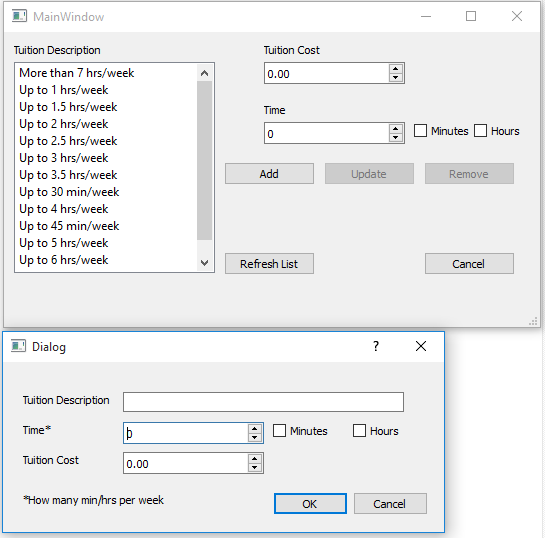
\includegraphics[scale=0.5]{tuitionRates.png}

\section{Teacher History}
This page includes several components. Firstly, user can use this page to find a specific teacher by entering a full or partial name of teachers. Secondly, users can click the history button to open up another window which has a list of classes the teacher has taught.\\

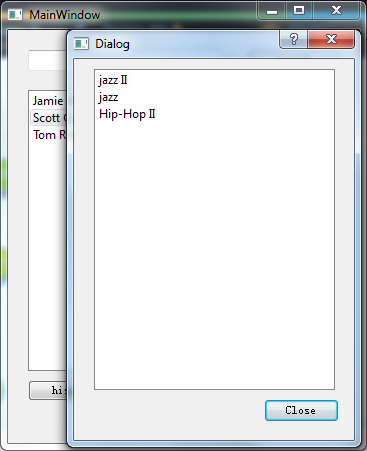
\includegraphics[scale=0.5]{teacherHistory.png}

\section{Set Semester}
This page helps users to set the current semester from pool of semester and add a new semester to the system.

\section{partial payment}
This page includes several components. Firstly, user can use this page to find a specific student by entering a full or partial name of students. Secondly, users can click the pay button to open up another window which asks user to input amount of money paid, payment's method and semester paid. The user also can choose single or multiple students at one time. \\
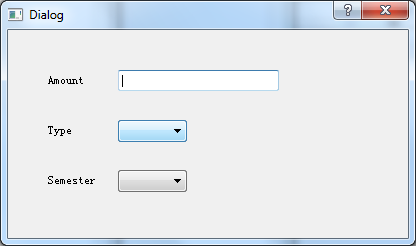
\includegraphics[scale=0.5]{payment.png}

\section{Student's owe}
This page includes several components. Firstly, user can use this page to find a specific student by entering a full or partial name of students. Secondly, users can click the statement button to open up another window which shows the amount of students paid, the amount of students due and the balance of student's account. Users also can print the invoice generated by the window.\\
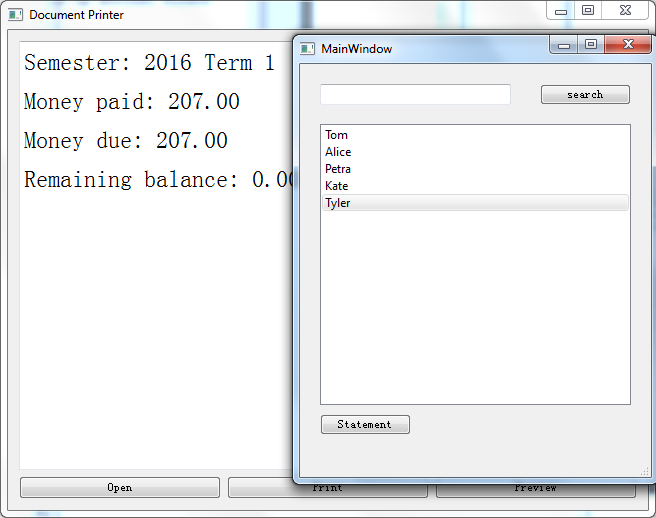
\includegraphics[scale=0.5]{invoice.png}

\section{enter payment}
This page includes several components. Firstly, user can use this page to find a specific student by entering a full or partial name of students. Secondly, users can click the clear button to clear the due of selected students. Users can select single or multiple students at one time.\\
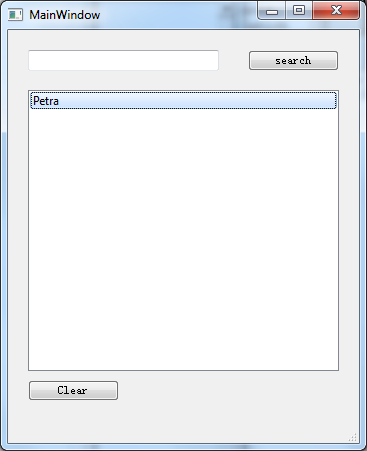
\includegraphics[scale=0.5]{enterPayment.png}

\section{bill history}
This page includes several components. Firstly, user can use this page to find a specific student by entering a full or partial name of students. Secondly, users can click the statement button in order to get the list of payments. In addition, user can print the bill history.\\

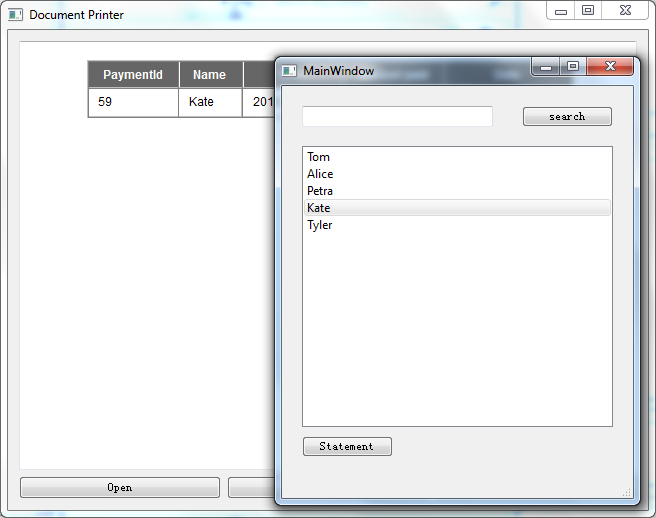
\includegraphics[scale=0.5]{billHistory.png}

\section{Sprint 3.5 and 4 Issues}
Some issues that were encountered during this sprint were:

\begin{enumerate}
\item During winter break the team wanted to tackle the student interface app. Building other required pages in the main local GUI made this a problem. Therefore while some implied GUI pages where fixed and created, the team was unable to get to the student interface. As a result the student interface was removed from the project requirements.
\item Spring semester ramp up - Coming back from a month break meant that the team needed to ramp back up and get used to the new classes and new commitments. This cause the team to move slower then it should have in this sprint. 
\item Team communication - The meeting this sprint were less effective as teams members would have other commitments, or in some cases lack the drive to do the work. This lessen as the sprint continued, but sometimes still came up.
\item Requirement Confusion - At times during this sprint the requirement were confusing. This resulted in a rewrite of the requires for payroll and billing to provide more clairity and adjust for dropping the student interface. The rework helped the team greatly, however the user stories still sometimes left out core part of how the academy does its work compared to other places. This resulted in spending more then the usually time speaking with the client, and group friction.
\end{enumerate}

\section{Client Interactions}

Client interactions came in the form of requires reviews and a demo of the prototype at the end of the sprint. Topics included:

\begin{enumerate}
\item Progress reports on where we are in the project
\item Asking questions to refine functionality, understand academy needs, and update requirements.
\item Discuss the future of the project and idea on how to execute them.
\item Prototype the current version of the prototype.
\end{enumerate}


\section{Group Meeting}

The group has a standard meeting time of TTH 10:00 - 12:00 and once during the weekend and at home as needed.  

Meeting can continue pass these times if needed, and other times during the weekend. However extra weekend times fluctuate and do not remain constant from week to week. 

\section{Work Distribution}

Marcus:
\begin{enumerate}
\item 3.5 Fix Assign Teacher Bug
\item 3.5 Update GUI Functions, Minor Additions and Fixes
\item 3.5 Tie Various Functions Into a Single Prototype
\item Prorated Refund (Still in Progress)
\item Enter Teacher Hours (Still in Progress)
\item Teacher Pay Rates (Needs Updated With New Information)
\item Early Registation Discounts
\item Gives Credits
\item Enter and Update Tuition Rates
\item Enter and Update Fee Rates and Type (Needs Updated With New Information)
\item documentation
\item trello management\\
\end{enumerate}

Dicheng:
\begin{enumerate}
\item 3.5 Class Search Pages
\item 3.5 Updated Role sheet
\item 3.5 Research Linux Boxes
\item 3.5 Tie Functions Together Into a Single Prototype
\item Enter Payments From Multiple Sources For One or More Students
\item Look at The Billing History
\item Enter a Full Payment For One or More Students
\item Enter Payments From Multiple Sources For One or More Students
\item Generate an invoice for the amount due (Needs Updated)
\item Look at a The Current Amount a Student/Family Owes
\item View Teaching History
\end{enumerate}


Together:
\begin{enumerate}
\item Updated database construction
\item GUI page breakdown based on user stories and product backlog
\item Coded some functionality
\end{enumerate}

\end{document}